\documentclass[11pt,a4paper,notitlepage,twocolumn]{article}

\usepackage[T1]{fontenc}
\usepackage[utf8]{inputenc}
\usepackage[english]{babel}
\usepackage{amsmath}
\usepackage{amsfonts}
\usepackage{amssymb}
\usepackage{verbatim}
\usepackage{listings}
\usepackage{color}
\usepackage{setspace}
\usepackage{epstopdf}
\usepackage{graphicx}
\usepackage{caption}
\usepackage{subcaption}
\usepackage{float}
\usepackage{epstopdf}
\usepackage{hyperref}
\usepackage{dsfont}
\usepackage{braket}
\pagenumbering{arabic}
\usepackage{titling}
\usepackage{fullpage}

\definecolor{codepurple}{rgb}{0.58,0,0.82}
\definecolor{backcolour}{rgb}{0.95,0.95,0.92}
\definecolor{dkgreen}{rgb}{0,0.6,0}
\definecolor{gray}{rgb}{0.5,0.5,0.5}
\definecolor{mauve}{rgb}{0.58,0,0.82}
%\setlength{\parindent}{0pt}

\lstdefinestyle{pystyle}{
  language=Python,
  aboveskip=3mm,
  belowskip=3mm,
  columns=flexible,
  basicstyle={\small\ttfamily},
  backgroundcolor=\color{backcolour},
  commentstyle=\color{dkgreen},
  keywordstyle=\color{magenta},
  numberstyle=\tiny\color{gray},
  stringstyle=\color{codepurple},
  basicstyle=\footnotesize,  
  breakatwhitespace=false
  breaklines=true,
  captionpos=b,
  keepspaces=true,
  numbers=left,
  numbersep=5pt,
  showspaces=false,
  showstringspaces=false,
  showtabs=false,
  tabsize=2
}
\lstdefinestyle{iStyle}{
  language=IDL,
  aboveskip=3mm,
  belowskip=3mm,
  columns=flexible,
  basicstyle={\small\ttfamily},
  backgroundcolor=\color{backcolour},
  commentstyle=\color{dkgreen},
  keywordstyle=\color{magenta},
  numberstyle=\tiny\color{gray},
  stringstyle=\color{codepurple},
  basicstyle=\footnotesize,  
  breakatwhitespace=false
  breaklines=true,
  captionpos=b,
  keepspaces=true,
  numbers=left,
  numbersep=5pt,
  showspaces=false,
  showstringspaces=false,
  showtabs=false,
  tabsize=2
}
\lstdefinestyle{c++style}{
  language=C++,
  keywordstyle=\color{blue}\ttfamily,
  stringstyle=\color{red}\ttfamily,
  commentstyle=\color{green}\ttfamily,
  morecomment=[l][\color{magenta}]{\#}
  aboveskip=3mm,
  belowskip=3mm,
  columns=flexible,
  basicstyle={\small\ttfamily},
  backgroundcolor=\color{backcolour},
  numberstyle=\tiny\color{gray},
  basicstyle=\footnotesize,  
  breakatwhitespace=false
  breaklines=true,
  captionpos=b,
  keepspaces=true,
  numbers=left,
  numbersep=5pt,
  showspaces=false,
  showstringspaces=false,
  showtabs=false,
  tabsize=2
}

\title{\normalsize Fys3150/4150 - Computational Physics\\
\vspace{10mm}
\huge 4. Ising model - Monte Carlo and Metropolis algorithms\\
\vspace{10mm}
\normalsize Due date {\bf Nov $overdue$, 2016}}

% Skriv namnet ditt her og fjern kommenteringa
\author{Magnus Christopher Bareid \\ un: magnucb }

\newcommand{\SE}{Schr\"odinger equation}
\newcommand{\laplacian}{\vec{\nabla}^2}
\newcommand{\eye}{\mathds{I}}
\newcommand\pd[2]{\frac{\partial #1}{\partial #2}}
\def\doubleunderline#1{\underline{\underline{#1}}}

\begin{document}
\noindent
\maketitle
\vspace{5mm}



%\begin{figure}[H]
%	\centering	
%	\includegraphics[scale=0.45]{frontpage.png}
%\end{figure}

%\begin{titlingpage}
%\begin{center}
\newpage
\begin{figure}[H]
\center
\includegraphics[scale=0.35]{../frontpage.png}
\end{figure}

\begin{abstract}
Empty void %TODO
\end{abstract}

\newpage
\tableofcontents

%\end{center}
%\end{titlingpage}

%\begin{center}
%\line(1,0){450}
%\end{center}


\newpage

\section*{Studies of phase transitions in magnetic systems}
\section{Introduction}
The aim of this project is to study a widely popular model to simulate phase transitions, the so-called Ising model in two dimensions. At a given critical temperature, this model exhbits a phase transition from a magnetic phase (a system with a finite magnetic moment) to a phase with zero magnetization.

As with all other projects in this course, the important thing is to make the algorithm work. The basic energy calculation of any two-dimensional lattice boils down to this form:
\begin{align}\label{eq:energysummation}
E = -J \sum^N_{<kl>} s_ks_l
\end{align}
where $s_k$ and $s_l$ are $\pm 1$ (up or down spin), $N$ is the total spins in the lattice, $J$ expresses the strength of interaction between neighbouring spins, which are referred to in the summation by $<kl>$ as it sums up interaction only between lattice-neighbours near index $k$ and $l$.

Through the course of this report, we shall investigate different variations on differently-sized lattices and their modelled physical properties.

\section{Analytical model of $2\times2$ lattice}
For our first trick, we shall simply investigate a $2\times2$ lattice of spins and its properties: its expectation value for energy and for absolute magnetic moment (mean magnetization), its  specific heat and magnetic susceptibility.

\subsection{The underlying math}
Firsly, we'll bee needing the partition function
\begin{align}\label{eq:partitionfunc}
Z = \sum_i e^{-\beta E_i}
\end{align}
where $E_i$ is a spin configuration's energy level, which $i$ counts over, and $\beta = 1/(k_B T)$ as a physical variable depending on temperature - a parameter which will become important in later sections.

The lattice's energy is given from the same form as equation (\ref{eq:energysummation}). The magnetic moment of such a lattice's spin combination is also important, and will yield values in a similar, but different pattern to the energy variations. For this we use:
\begin{align}\label{eq:magnetsummation}
M = \sum_{i=1}^N s_i
\end{align}
where $M_i$ signifies a lattice location's spin orientation. This reveals to us a set of energies and magnetizations that the $2\times2$ lattice and its possible spin configurations may yield.
\begin{table}[H]
\center
\begin{tabular}{|c|c|r|r|} \hline

	\# $s_i=$ 1 & \# states & E & M  \\ \hline
	4 & 1 & -8J & 4   \\
	3 & 4 & 0   & 2   \\
	2 & 4 & 0   & 0   \\
	2 & 2 & 8J  & 0   \\
	1 & 4 & 0   & -2  \\
	0 & 1 & -8J & -4  \\ \hline
\end{tabular}
\caption{Overview over how number of spins in a direction determines energy and magnetization of a lattice, and its multiplicity.}\label{table:spincombinations}
\end{table}

For the related expectation values, these are formed by multiplying by the probability of each state, which is determined with a natural exponent and the partition function that we elaborated earlier:
\begin{align}\label{eq:exvals}
<E^n> &= \frac{1}{Z}\sum_i E_i^n e^{-\beta E_i}  \\
<|M|^n> &= \frac{1}{Z}\sum_i M_i^n e^{-\beta E_i} \nonumber
\end{align}
where $i$ iterates over all possible combinations - not over all locations in a lattice.

Furthermore, the formulation for specific heat and magnetic susceptibility reads thus:
\begin{align}\label{eq:specheat_magsus}
C_V &= \frac{<E^2> - <E>^2}{k_B T^2} \\
\chi &= \frac{<M^2> - <M>^2}{k_B T} \nonumber
\end{align}

\subsection{Results}
When all of these energy and magnetic combinations are input to a simple python script, the analytical values which we were supposed to investigate, as mentioned in the beginning of the section, may be evaluated:

\begin{table}[H]
\center
\begin{tabular}{|c|r r|}\hline
	$<E>$ &-7.98392834375   $\approx$ & -7.9839\\ \hline
	$<M>$ & 3.99464293099   $\approx$ & 3.9946\\ \hline
	$C_V$ & 0.128329327457  $\approx$ & 0.12833\\ \hline
	$\chi$& 0.0160429580649 $\approx$ & 0.016043\\ \hline
\end{tabular}
\caption{Analytical values as determined by a python script.}\label{table:analyticalresults}
\end{table}

\section{Making a working numerical model for a $2\times2$ lattice}
Now comes the fun part% DIE DIE DIE!!!!!!!!
, modelling the previous system numerically, using Monte Carlo style in C++.

\subsection{How the script works}
The script begins by taking in several values of the lattice system, such as lattice length, how many Monte Carlo cycles which we will cycle the system over, temperature for the lattice to hold. The temperature in this case is set to 1 for simplicity's sake. Physical units and confusions apply.

Then the inital lattice matrix is set up with corresponding energy and magnetization quantities; for this problem's purposes we simply start with all spins up.

At every iteration of the Monte Carlo cycle, the lattice is adjusted according to principles of physics: A random spin is chosen to turn its value. If the new energy state has less energy than the previous one, the new energy state is then accepted its new properties for energy and magnetization are applied to the system.

Expectation values are yielded from dividing by number of Monte Carlo cycles which the system has had to go through in order to achieve its current properties. The iterated values are stored to data files for later use, expectation values are printed to screen along with specific heat and magnetic susceptibility.

\subsection{Results and discussion}\label{disc:ana_results}
A run for several Monte Carlo simulation lengths yielded these values, which are compared with analytical results as shown in table \ref{table:analyticalresults}.
\begin{table}[H]\center
\begin{tabular}{|c|r|r|}\hline
	Quant.& Result & $\approx\Delta$ Ana.\\ \hline
	$<E>$ &-7.2    & 0.7839 \\ \hline
	$<M>$ & 3.63   & 0.3646 \\ \hline
	$C_V$ & 5.76   & 5.632 \\ \hline
	$\chi$& 1.44   & 1.424 \\ \hline
\end{tabular}
\caption{Results after $10^1$ Monte Carlo cycles.}\label{table:4bresults10}
\begin{tabular}{|c|r|r|}\hline
	Quant.& Result & $\approx\Delta$ Ana.\\ \hline
	$<E>$ &-7.92   & 0.0639 \\ \hline
	$<M>$ & 3.96   & 0.0346 \\ \hline
	$C_V$ & 0.6336   & 0.5053 \\ \hline
	$\chi$& 0.1584   & 0.1423 \\ \hline
\end{tabular}
\caption{Results after $10^2$ Monte Carlo cycles.}\label{table:4bresults100}
\begin{tabular}{|c|r|r|}\hline
	Quant.& Result & $\approx\Delta$ Ana.\\ \hline
	$<E>$ &-7.984  & 0.0001 \\ \hline
	$<M>$ & 3.992  & 0.0026 \\ \hline
	$C_V$ & 0.127744 & 0.0006 \\ \hline
	$\chi$& 0.031936 & 0.0159 \\ \hline
\end{tabular}
\caption{Results after $10^3$ Monte Carlo cycles.}\label{table:4bresults1000}
\begin{tabular}{|c|r|r|}\hline
	Quant.& Result & $\approx\Delta$ Ana.\\ \hline
	$<E>$ &-7.9856    & 0.0017 \\ \hline
	$<M>$ & 3.995    & 0.0004 \\ \hline
	$C_V$ & 0.114993   & 0.0133 \\ \hline
	$\chi$& 0.015575   & 0.0005 \\ \hline
\end{tabular}
\caption{Results after $10^4$ Monte Carlo cycles.}\label{table:4bresults10000}
\begin{tabular}{|c|r|r|}\hline
	Quant.& Result & $\approx\Delta$ Ana\\ \hline
	$<E>$ &-7.982  & 0.0019 \\ \hline
	$<M>$ & 3.99396    & 0.0007 \\ \hline
	$C_V$ & 0.143676   & 0.0153 \\ \hline
	$\chi$& 0.0182035   & 0.0022 \\ \hline
\end{tabular}
\caption{Results after $10^5$ Monte Carlo cycles.}\label{table:4bresults100000}
\end{table}
\begin{table}
[H]\center
\begin{tabular}{|c|r|r|}\hline
	Quant.& Result & $\approx\Delta$ Ana.\\ \hline
	$<E>$ &-7.98436 & 0.0004 \\ \hline
	$<M>$ & 3.99479 & 0.0001 \\ \hline
	$C_V$ & 0.124875 & 0.0035 \\ \hline
	$\chi$& 0.0156048 & 0.0004 \\ \hline
\end{tabular}
\caption{Results after $10^6$ Monte Carlo cycles.}\label{table:4bresults1000000}
\end{table}

It would seem that already after having passed 10$^3$ Monte Carlo cycles, the accuracy starts to become surprisingly impressive, and varies less. However, the clear trend is of course that the more one increases the number of cycles for the program to run through, the more accurate results. My own verdict would claim that any run of the script with more than 10$^6$ Monte Carlo cycles would be accurate enough for most purposes.

\section{When a $20\times20$ lattice reach equilibrium}
Now, let us try to expand our system and investigate some properties that follow. We expand the lattice by a factor of 10 in both dimensions. To find out how this system behaves, it is interesting to investigate how quickly it reaches its equilibrium state, and to investigate if the corresponding phenomena's changes are temperature dependant. 
\subsection{Modifying the script}
In order to achieve this, we will have to modify the script slightly. The aforementioned C++ script gains an if-test which initializes correct values for the lattice initialization, and then models the lattice as previously - once per temperature variation. For the purposes of this investigation, a range of 8 temperature values between 1 and 2.4 were chosen.
\subsection{Spin-up orientation results}
For a $20\times20$ spin lattice system, 1.2 $\cdot 10^4$ Monte Carlo cycles, with an initial spin-up oriention, for a range of temperatures, the below plots were produced.

All expectation values are normalized to the corresponding expectation value's final calculated value, which would be the corresponding expectation value's nearest value to the analytical value.
\begin{figure}
[H]\center
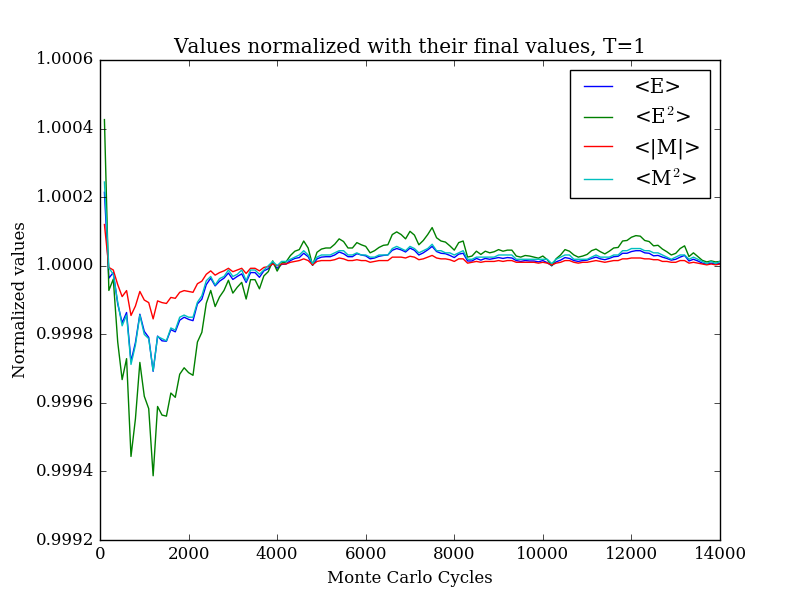
\includegraphics[scale=0.35]{../figs/4c/Prob_L20_mc100000_T100_spinup.png}
\caption{A normalized mean energy and magnetic moment view of the iterated evolution of the spin lattice at temperature value of 1.}
\end{figure}
\begin{figure}
[H]\center
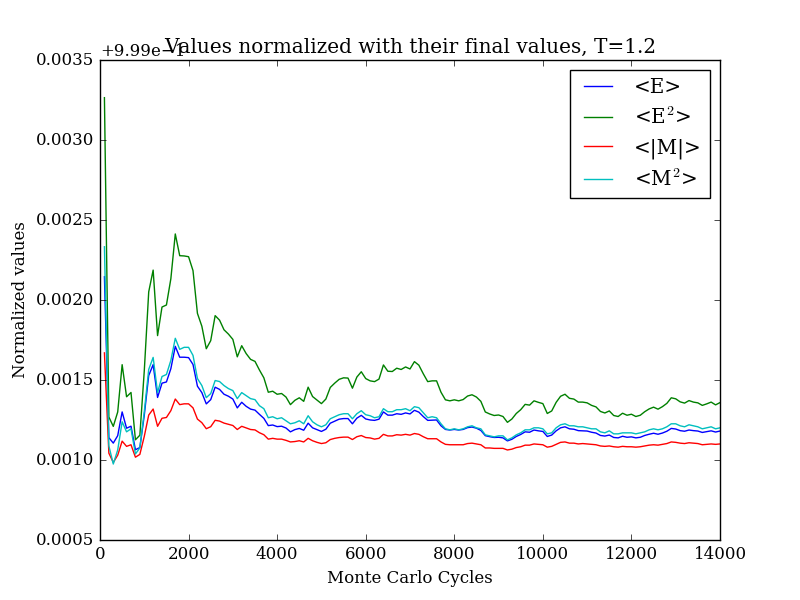
\includegraphics[scale=0.35]{../figs/4c/Prob_L20_mc100000_T120_spinup.png}
\caption{A normalized mean energy and magnetic moment view of the iterated evolution of the spin lattice at temperature value of 1.2.}
\end{figure}
\begin{figure}
[H]\center
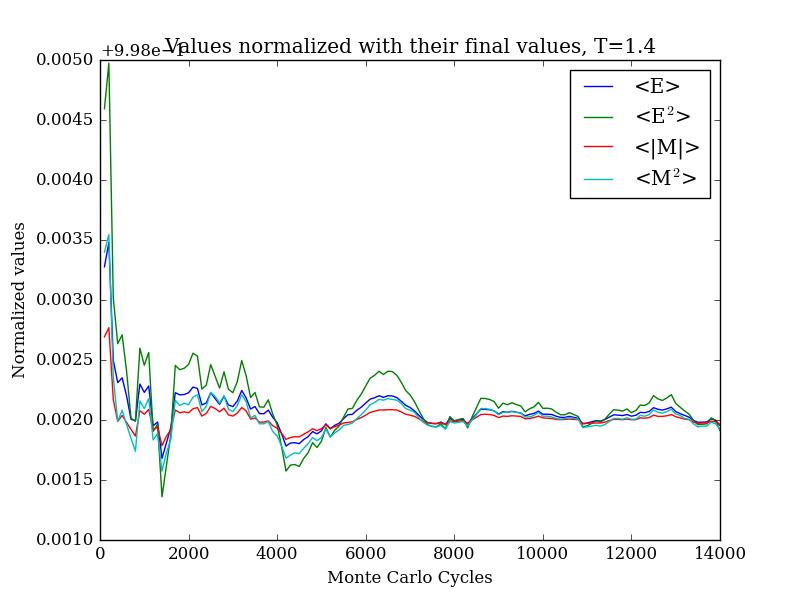
\includegraphics[scale=0.35]{../figs/4c/Prob_L20_mc100000_T140_spinup.png}
\caption{A normalized mean energy and magnetic moment view of the iterated evolution of the spin lattice at temperature value of 1.4.}
\end{figure}
\begin{figure}
[H]\center
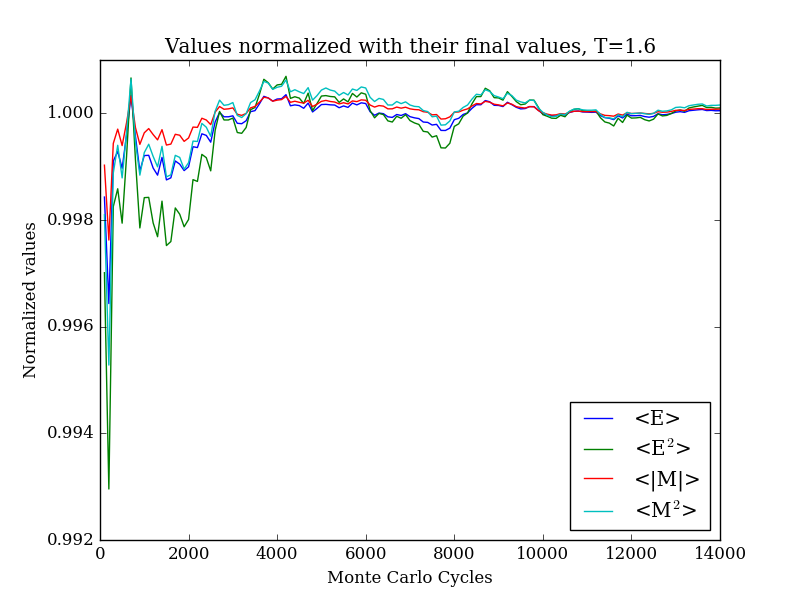
\includegraphics[scale=0.35]{../figs/4c/Prob_L20_mc100000_T160_spinup.png}
\caption{A normalized mean energy and magnetic moment view of the iterated evolution of the spin lattice at temperature value of 1.6}
\end{figure}
\begin{figure}
[H]\center
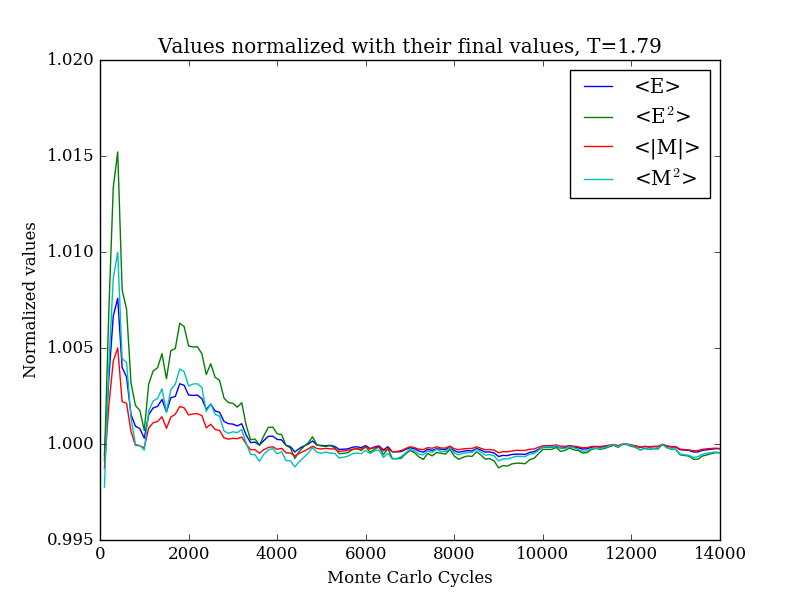
\includegraphics[scale=0.35]{../figs/4c/Prob_L20_mc100000_T179_spinup.png}
\caption{A normalized mean energy and magnetic moment view of the iterated evolution of the spin lattice at temperature value of 1.79}
\end{figure}
\begin{figure}
[H]\center
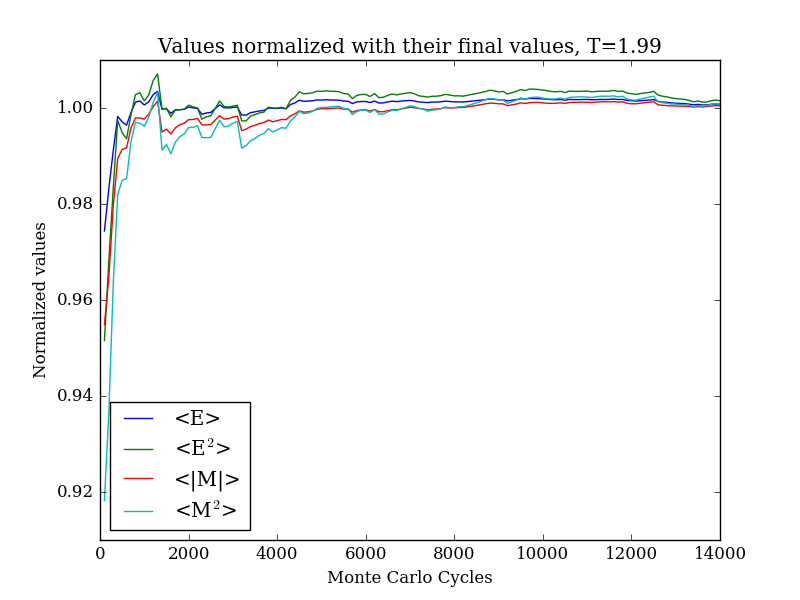
\includegraphics[scale=0.35]{../figs/4c/Prob_L20_mc100000_T199_spinup.png}
\caption{A normalized mean energy and magnetic moment view of the iterated evolution of the spin lattice at temperature value of 1.99}
\end{figure}
\begin{figure}
[H]\center
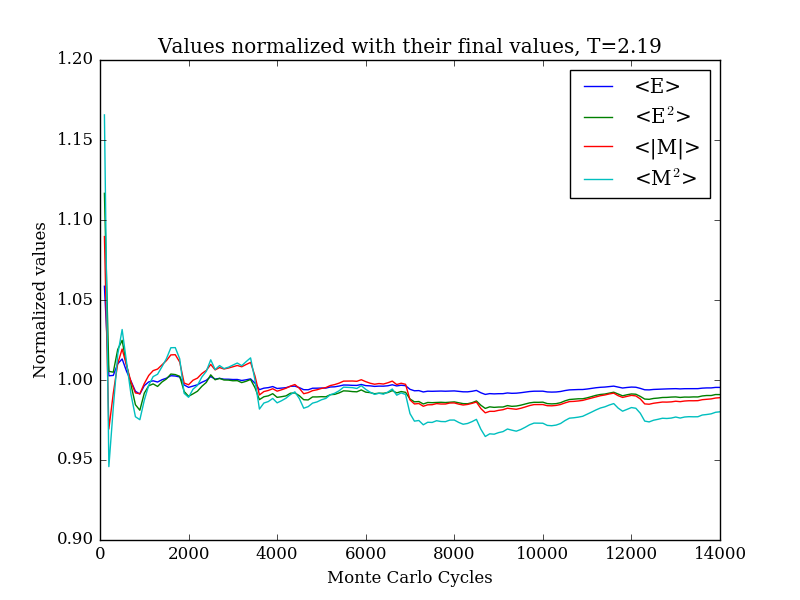
\includegraphics[scale=0.35]{../figs/4c/Prob_L20_mc100000_T219_spinup.png}
\caption{A normalized mean energy and magnetic moment view of the iterated evolution of the spin lattice at temperature value of 2.19}
\end{figure}
\begin{figure}
[H]\center
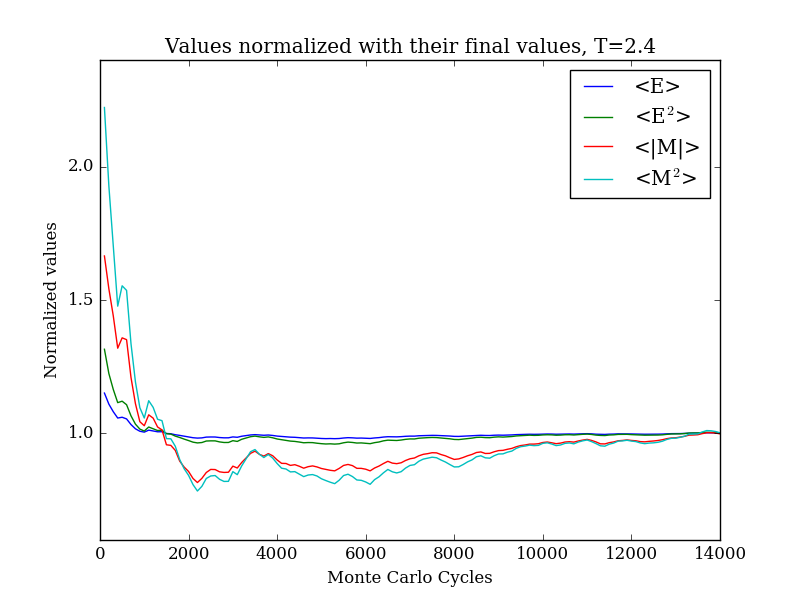
\includegraphics[scale=0.35]{../figs/4c/Prob_L20_mc100000_T240_spinup.png}
\caption{A normalized mean energy and magnetic moment view of the iterated evolution of the spin lattice at temperature value of 2.40.}
\end{figure}
\subsection{Spin-up orientation discussion}
When one looks closely at the above section's produced plots, one can see a clear trend that the expectation values' slope smoothes out quite dominantly already at around 13 000 Monte Carlo cycles.
\subsection{Random spin orientation results}
For a $20\times20$ spin lattice system, 1.2 $\cdot 10^4$ Monte Carlo cycles, with an initial randomized spin oriention, for a range of temperatures, the below plots were produced.

All expectation values are normalized to the corresponding expectation value's largest value.
\begin{figure}
[H]\center
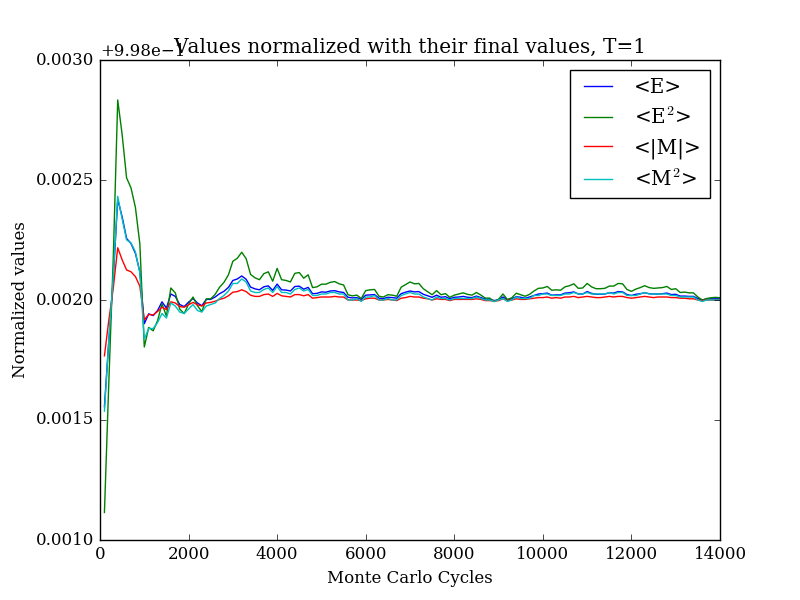
\includegraphics[scale=0.35]{../figs/4c/Prob_L20_mc100000_T100_spinrandom.png}
\caption{A normalized mean energy and magnetic moment view of the iterated evolution of the spin lattice at temperature value of 1.}
\end{figure}
\begin{figure}
[H]\center
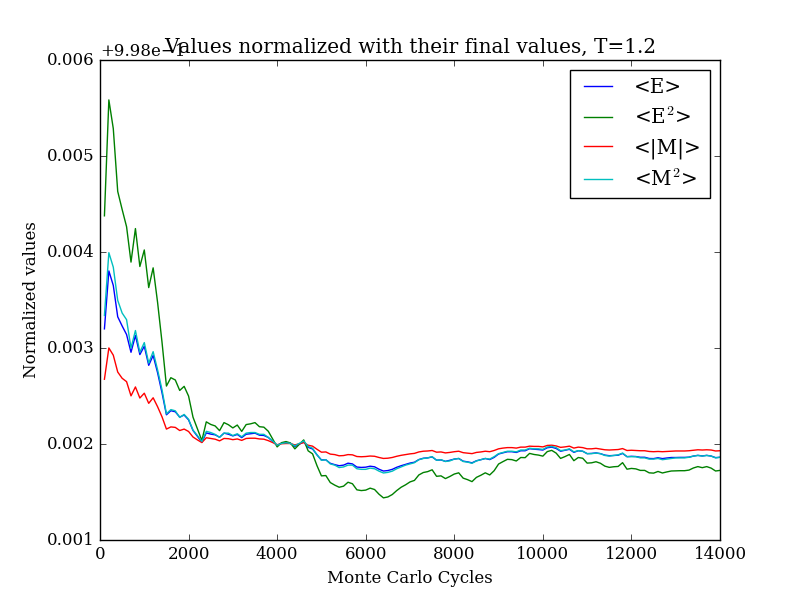
\includegraphics[scale=0.35]{../figs/4c/Prob_L20_mc100000_T120_spinrandom.png}
\caption{A normalized mean energy and magnetic moment view of the iterated evolution of the spin lattice at temperature value of 1.2.}
\end{figure}
\begin{figure}
[H]\center
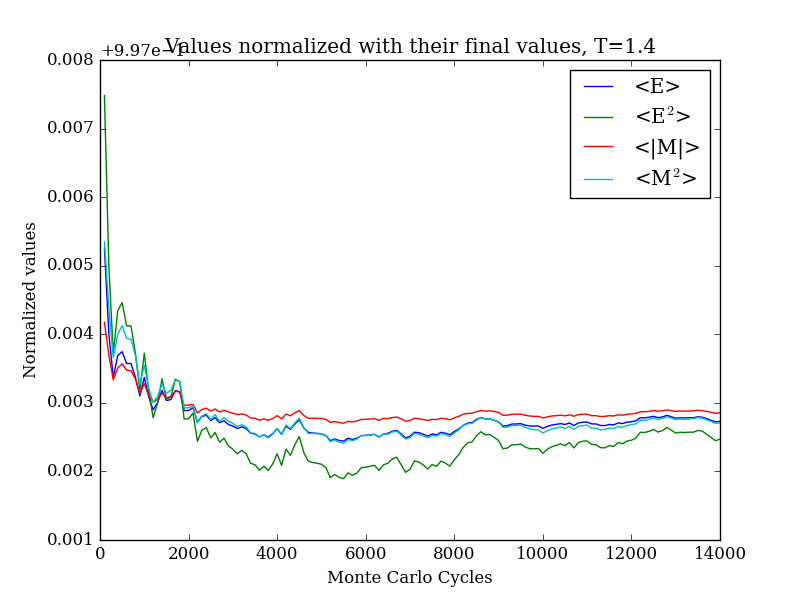
\includegraphics[scale=0.35]{../figs/4c/Prob_L20_mc100000_T140_spinrandom.png}
\caption{A normalized mean energy and magnetic moment view of the iterated evolution of the spin lattice at temperature value of 1.4.}
\end{figure}
\begin{figure}
[H]\center
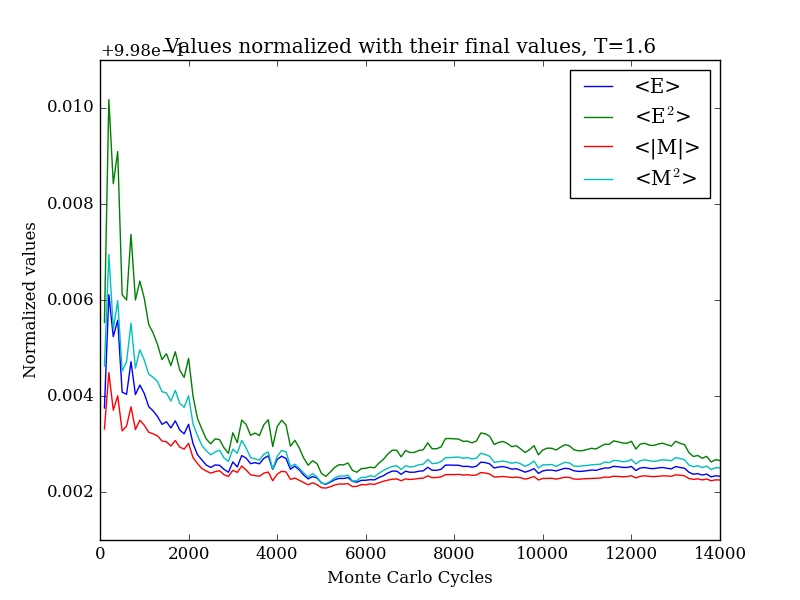
\includegraphics[scale=0.35]{../figs/4c/Prob_L20_mc100000_T160_spinrandom.png}
\caption{A normalized mean energy and magnetic moment view of the iterated evolution of the spin lattice at temperature value of 1.6}
\end{figure}
\begin{figure}
[H]\center
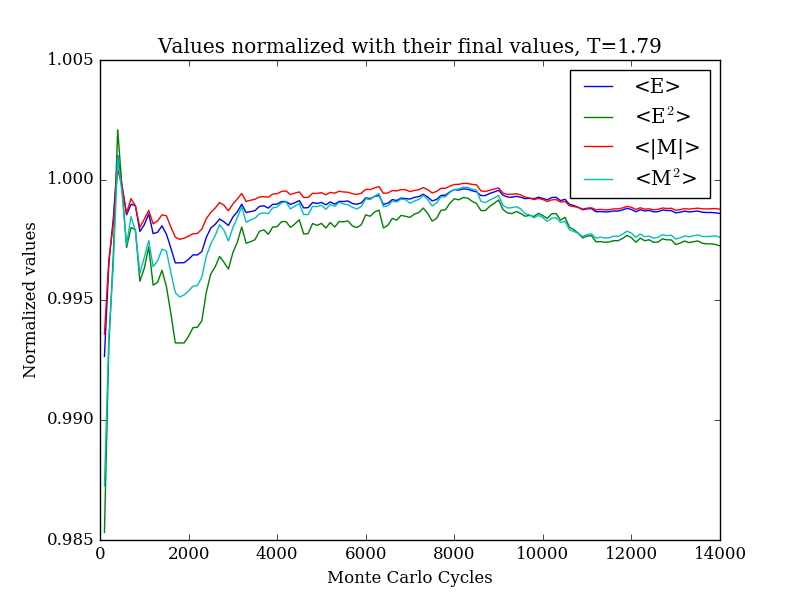
\includegraphics[scale=0.35]{../figs/4c/Prob_L20_mc100000_T179_spinrandom.png}
\caption{A normalized mean energy and magnetic moment view of the iterated evolution of the spin lattice at temperature value of 1.79}
\end{figure}
\begin{figure}
[H]\center
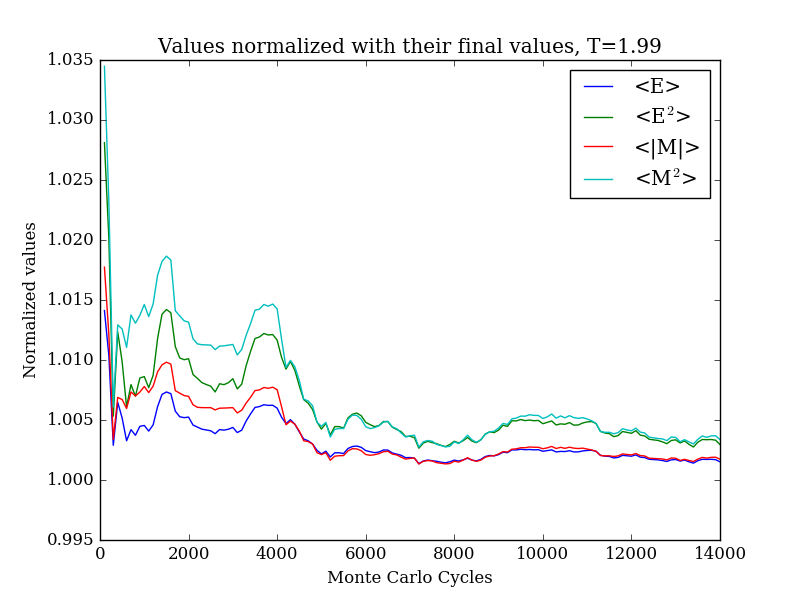
\includegraphics[scale=0.35]{../figs/4c/Prob_L20_mc100000_T199_spinrandom.png}
\caption{A normalized mean energy and magnetic moment view of the iterated evolution of the spin lattice at temperature value of 1.99}
\end{figure}
\begin{figure}
[H]\center
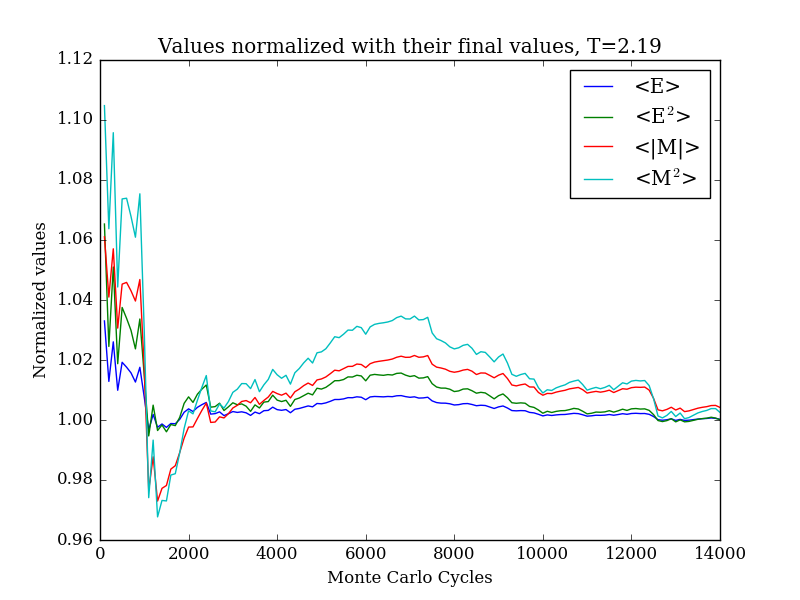
\includegraphics[scale=0.35]{../figs/4c/Prob_L20_mc100000_T219_spinrandom.png}
\caption{A normalized mean energy and magnetic moment view of the iterated evolution of the spin lattice at temperature value of 2.19}
\end{figure}
\begin{figure}
[H]\center
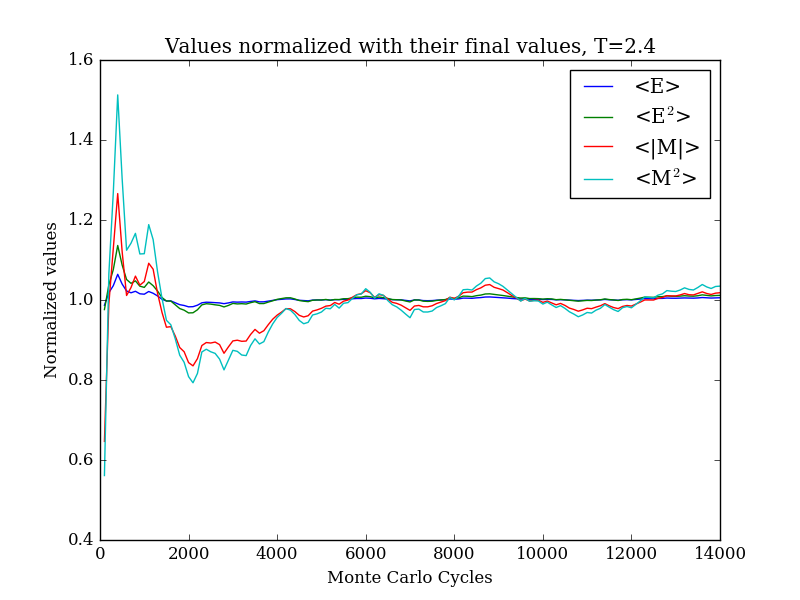
\includegraphics[scale=0.35]{../figs/4c/Prob_L20_mc100000_T240_spinrandom.png}
\caption{A normalized mean energy and magnetic moment view of the iterated evolution of the spin lattice at temperature value of 2.40.}
\end{figure}
\subsection{Random spin orientation discussion}\label{disc:stabilize}
As with before, when one look closely at the above section's produced plots, one can see a clear trend that the expectation values' slope smoothes out quite dominantly already at around 13 000 Monte Carlo cycles.

Some of the systems start off way more erratic, but their behavioural trend still seems very clear: the variation of every system seems to decrease as the system evolves, and for our intents and purposes it seems to stabilize sufficiently after around 13 000 Monte Carlo cycles.

\subsection{Accepted energy shifts}
Another way to perceive how when a system reaches an equilibrium state, is to investigate when it stops changing. As aforementioned in how the script works, the way this model evolves is to attempt a new lattice's spin configuration and check if this new spin configuration yields a valid energy state of the lattice. If this check passes, the new configuration is accepted as a physical state according to the entropic principle, and the spin configuration's energy state is applied.

By tracking how often a new configuration is applied, it should show where an equilibrium state is reached by determining at which point in the Monte Carlo evolution that the lattice stops evolving - if it reaches a definite equilibrium point. If the lattice isn't able to reach this equilibrium point exactly, intuitively it should continue to evolve with oscillations around the equilibrium point, until the lattice eventually may land on an exact equilibrium point.

\subsection{Results and discussion of accepted configurations' investigation}\label{disc:accepted}
A plotting of the total number of spin configurations on Monte Carlo evolution produced these two plots, one for each initial spin orientation, with all temperatures included.
\begin{figure}
[H]\center
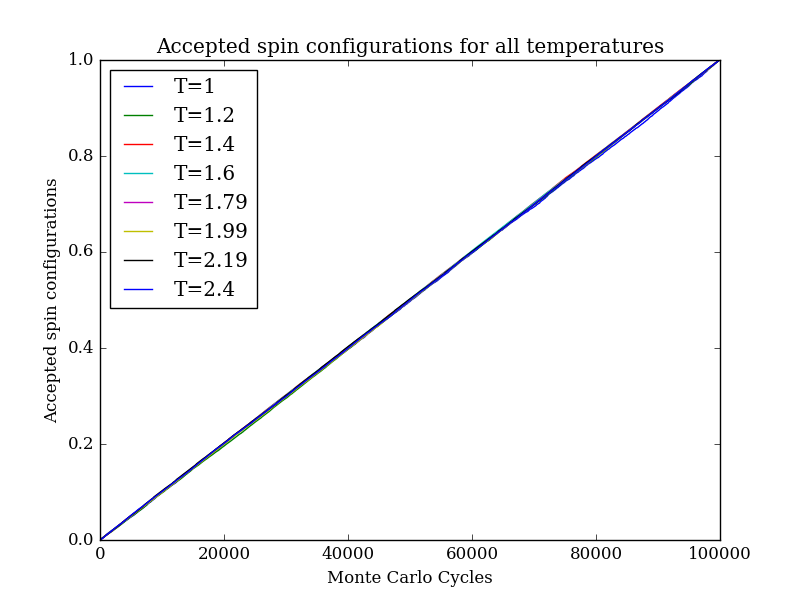
\includegraphics[scale=0.35]{../figs/4c/acceptedspins_up.png}
\caption{A tracking of accepted number of configurations over total Monte Carlo cycles for all temperatures, with initial spin orientation as up.}
\end{figure}
\begin{figure}
[H]\center
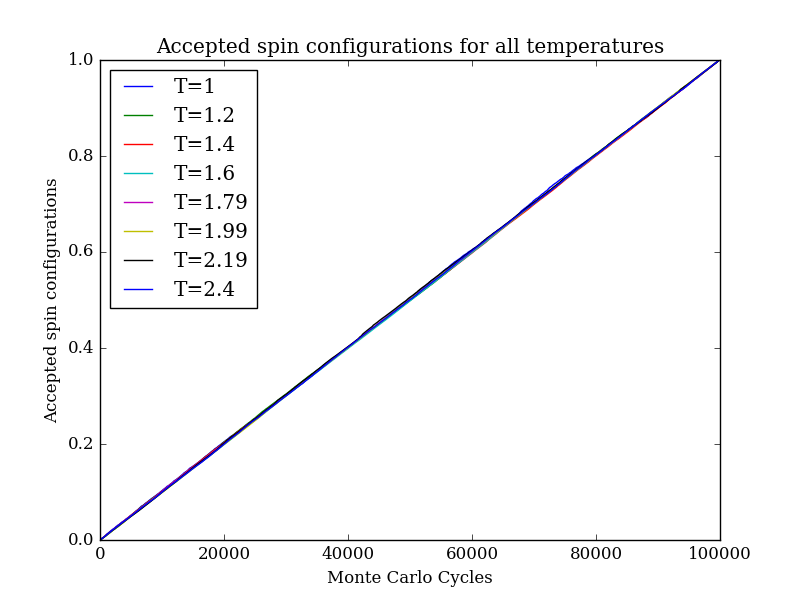
\includegraphics[scale=0.35]{../figs/4c/acceptedspins_random.png}
\caption{A tracking of accepted number of configurations over total Monte Carlo cycles for all temperatures, with initial spin orientation as random.}
\end{figure}
As the plots show for both initial spin configurations, the number of accepted spin configurations increase steadily with a constant slope for all temperatures. This seems to indicate that even if the expectation values seem to reach the neighbourhood of an equilibrium point, as indicated by the previous plots, these plots show that the lattice's expectation values continue to oscillate around their expectation values, instead of landing on final values.

As another point worthy of note, one could investigate how the total number of spin configurations behave for the different temperature sets.
\begin{figure}
[H]\center
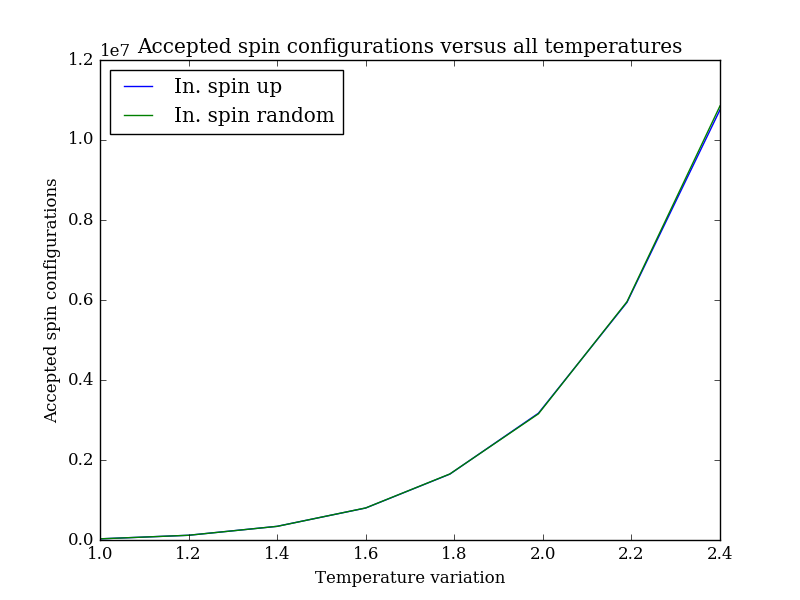
\includegraphics[scale=0.35]{../figs/4c/acceptedspins_vsTemps.png}
\caption{A visualization of how many accepted spin configurations exist for each temperature variation.}
\end{figure}
\begin{figure}
[H]\center
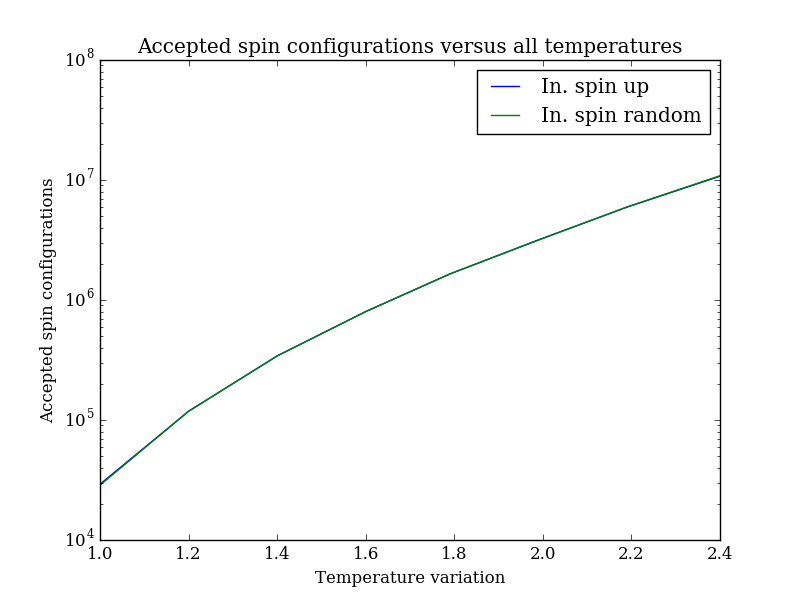
\includegraphics[scale=0.35]{../figs/4c/acceptedspins_vsTemps_log.png}
\caption{A visualization of how many accepted spin configurations exist for each temperature variation, accepted spin configuration count log scaled.}
\end{figure}
The two above figures clearly indicate that there are significantly more acceptable spin configurations with increasing temperature for the lattice structure. This means that for a higher temperature setting, the lattice may arrange its spins in significantly more ways that would oscillate around an equilibrium point, even for slight increases in temperatures.

It is also worth noting that the simulated lattices' number of accepted configurations are virtually identical for both an upwards ordered or a randomly ordered initial spin configurations, for all temperatures. This is probably due to the observation and statement that the lattice's configuration system begins to oscillate at a fairly early stage, thus smoothing out differences from initial configurations that for shorter simulations seem much more dominant.

\section{Making a probability estimate of an energy quantity}
Through all the oscillations of the lattice's spin configurations, some total energies are bound to appear more than once, thus yielding a system of more or less probable energy states, telling us what quantities of energy the lattice would oscillate around.

To achieve this, some modifications on the C++ script need to be done.

\subsection{Modifying the script}
An if-test is added to the section of the Monte Carlo cycle iteration, so that the necessary values may be stored to a new file - in this case we are not looking for the expectation values themselves, but rather the current energy level and its variance at each iterative step through the time evolution of the lattice.

\subsection{Results and discussion of the probabilities}
Making a histogram over the energies for an initially upwards and random orientied spin configuration lattice produced the below figures.
\begin{figure}
[H]\center
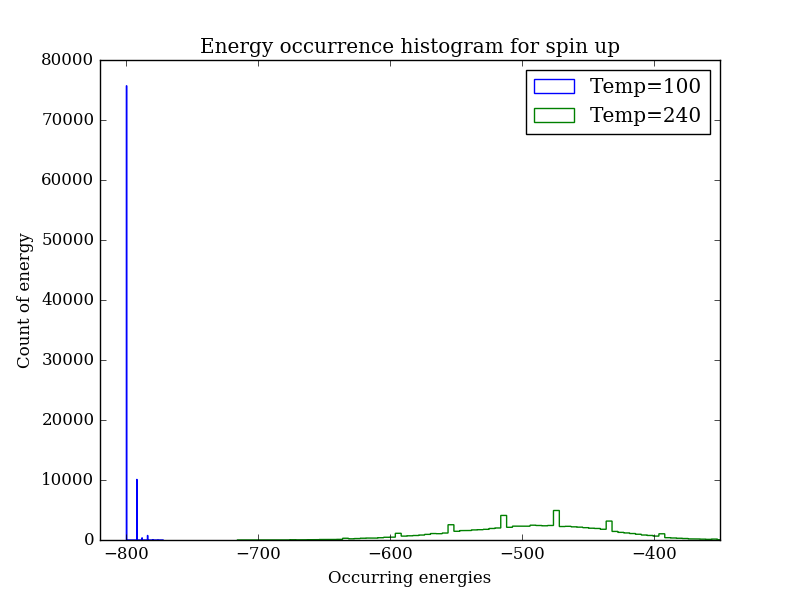
\includegraphics[scale=0.35]{../figs/4d/probabilityhistogram_up.png}
\caption{Energy level histogram for the lattice's time evolution after stabilization, upwards initial spin configuration.}
\end{figure}
\begin{figure}
[H]\center
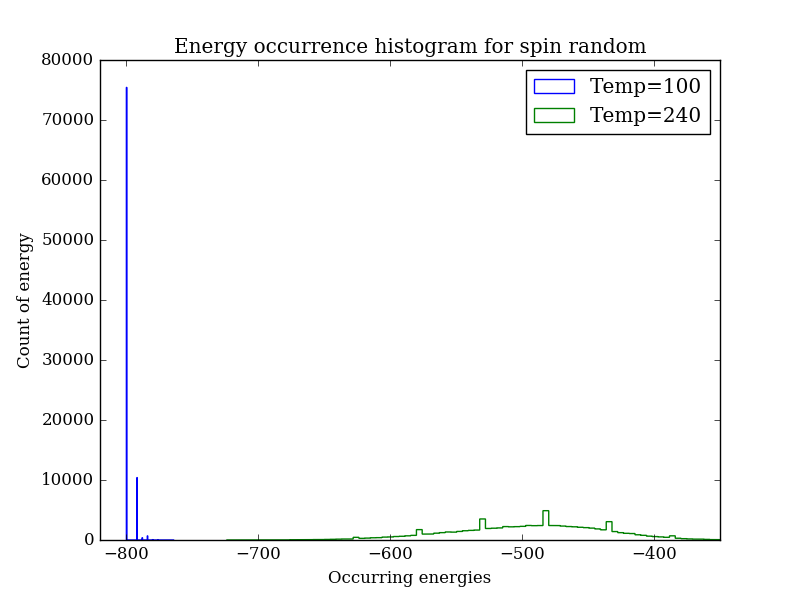
\includegraphics[scale=0.35]{../figs/4d/probabilityhistogram_random.png}
\caption{Energy level histogram for the lattice's time evolution after stabilization, random initial spin configuration.}
\end{figure}
For the upward initial spin configuration, this is the collected data - the numbers have been truncated slightly to increase readability:

\begin{table}
[H]
\begin{tabular}{|c|c|r|r|r|r|}\hline
	Spin & T= & En. & \# count & $P(E)$ & $\sigma_E$ \\ \hline
	Up & 1.0 & -798.0 & 75705 & 0.870 & 9.481\\ \hline 
	Up & 2.4 & -494.0 & 4767 & 0.055 & 3286 \\ \hline
	Ran. & 1.0 & -798.0 & 5432 & 0.867 & 9.483 \\ \hline
	Ran. & 2.4 & -506.0 & 4420 & 0.051 & 4420\\ \hline
\end{tabular}
\caption{Table of energy levels' counts and their probabilities of occuring in the lattice.}
\end{table}
From these graphs and computed data one may suppose that the system oscillates around certain values, and increasingly lands on different values around its oscillation point with increased temperature - just as I suggested in section \ref{disc:accepted}.

Moreover, the fact that the different initial orientations' direction seem to make no difference to the results further solidifies that the lattices will oscillate around a common energy level, or at least an energy level that is in the neighbourhood of each other. It would seem intuitive with the reasoning used up until now that the lower the temperature setting, then the closer will the lattice's common oscillation point be, as per the above table.

The interesting part of these data, however, is the deviance between the high-temperature lattices' variance in energy. For the initially randomized spin configuration lattice, the variance is significantly larger than the initially upward oriented spin configuration lattice. The variance is an inherent part of the data, related to the full width of half maximum of the distribution, and this point suggests that the randomized lattice has a broader spectrum of oscillatory energy levels at which the lattice lands, further suggesting that 13 000 Monte Carlo cycles may not be enough time to stabilize this high-temperature lattice, as concluded per section \ref{disc:stabilize}.

As a huge \textbf{PS} from my part: as of trouble-shooting this section, I found that the printouts of section  \ref{disc:ana_results} may have had some bad values for the heat capacity $C_V$. I'm not sure what exactly was wrong, for as of calculating the current section's values, well, the numbers that I got were only slightly off from the desired values, and I stumbled over a way of fixing all of it without noticing exactly what I did that fixed it. It works now, though! But the values of that section is too much a bother to re-evalutate, and the following sections' plots are normalized in such a way the behaviour of the heat capacity's graphs should remain identical to what they looked like, even with off-set numbers underlying the scaling, so I choose to go forward with the tasks, rather than knit-pick with trifles.

\section{Appendix}
\subsection{Code and GitHub}
All my code is located at this address:

\url{https://github.com/magnucb/p4}

\begin{thebibliography}{9}
\bibitem{example_code}
  Jensen, M 2016,
  \verb|ParaIsingModel.cpp|,
  
  viewed $22^{th}$ of November 2016,
  \url{https://github.com/CompPhysics/ComputationalPhysics/blob/master/doc/Programs/ParallelizationMPI/ParaIsingModel.cpp}.
  
\bibitem{analytical_methods}
	Jensen, M 2016, 
	Computational Physics Lecture Notes Fall 2015:
	
	13.2.2: Canonical Ensemble \& 
	
	13.3.1: Ising Model and Phase Transitions in Magnetic Systems,
	
	viewed $22^{th}$ of November 2016, 
	\url{http://compphysics.github.io/ComputationalPhysics/doc/Lectures/lectures2015.pdf}

\end{thebibliography}

\end{document}